%\dropchapter{0.4in}
\chapter{Anomalous couplings in top physics} \label{chp::SM}
%\epigraphhead[70]{\epigraph{\textit{If I could remember the names of all these particles, I'd be a botanist.}}{Enrico Fermi}}
%\undodrop

%The ultimate goal of any particle physics is to \\
%Within experimental particle physics, the ultimate goal is to understand \\
%(Ever since the beginning of physics, and especially of particle physics, the ultimate goal is to progress and move forward in the understanding of the particles and their interactions observed around us. )
%In order to achieve a new breakthrough on the level of elementary particle physics our current knowledge should continously be questioned and no detail, no matter how small, should be overlooked.
%** no stone should be left unturned **.
%In this perspective the Standard Model of elementary particle physics should be seen as a first step towards a grand unification of all fundamental interactions which has met every test endured up to now.
%endured is ``tested to the limit'' time after time, but for the moment has met every test.
%\\
%\textit{Now shortly summarize what will be discussed in this chapter!}\\
%\textbf{More focus ont he role of top in SM searches!}

The ultimate goal of elementary particle physics is achieving a complete and profound understanding of the most elementary parts of the elements surrounding us, and preferably doing so with a single theory.
The quest to such a ``theory of everything'' led to the development of the Standard Model of elementary particle physics, which can be seen as a first step towards a grand unification of all fundamental interactions. %has met every test endured up to now ...
The most important aspects of the Standard Model, particle content and theoretical framework, are discussed first in detail in Section~\ref{sec::SM}.
\\
\\
Further emphasis will be laid on the particularities of the top quark, the heaviest quark existing within the Standard Model, which plays an important role in assessing the Standard Model at high energies. 
Hence this sector is extremely interesting to search for influences of new physics phenomena, for example in the shape of anomalous couplings as will be discussed in Section~\ref{sec::TopQuarkPhysics}.

\section{Standard Model of elementary particle physics} \label{sec::SM}
The Standard Model of elementary particle physics (SM) is a theoretical framework designed in 1978, which contains three of the four fundamental interactions.

\subsection{Particle content}

The exhaustive inquiry performed during the 20$^{th}$ century to define the elementary particles and the corresponding discoveries continously altered the understanding of the fundamental interactions.
%It almost appears that every new particle discovery resulted in a complete destruction of the existing theory assumptions.
Every new achievement divided the physics community and often required the development of a brand new framework capable of describing the observations.
Hence the Standard Model, officially established in the early 1970s, actually consists of many ingenious contributions from many renown physicists~\cite{MandlAndShaw, PeskinAndSchroeder, Paschos:2007pi}. 
For the last decades the general belief on elementary particles is considered rather stable, especially since every new discovery validated the Standard Model. % and summarized in Table~\ref{table::ElemParticles}.
\\

Within the Standard Model the elementary particles are categorized based on their spin. Fermions, containing both leptons and quarks, have half-integer spin while bosons, also called force mediators, have integer spin. 
The collection of fermions can be stored into three separate generations, characterized by increasing mass, as shown in Table~\ref{table::ElemParticles}.  Each fermion $f$ has an antiparticle, which is defined to have identical mass but opposite electrical charge and is generally denoted as $\bar{f}$. 
Only for the charged leptons, $l^{-}$, the notation $l^{+}$ is used for their respective antiparticle.
\\
Even though the Standard Model consists of three fermion generations the first one is sufficient to describe all stable matter around us.
This because a single atom consists of an electron circulating around a proton-neutron nucleus, which are bound states of up- and down-quarks with respective quark-content $uud$ and $udd$. From such an atom every known chemical element can be formed. 
%This because the protons and neutrons are a bound state of up- and down-quarks, respectively with quark-content $uud$ and $udd$. Together with the electron circulating around the proton-neutron nucleus this gives rise to a simple atom from which every known chemical element can be formed. 
\setlength\extrarowheight{5pt}
\begin{table}[h!t]
 \centering
 \caption{Overview of the fermions in the Standard Model and their corresponding electrical charge.} \label{table::ElemParticles}
 \begin{tabular}{|c|cr|cc|cc|cc|c|}
  \hline
  \textbf{Generation} 		& \multicolumn{4}{c|}{\textbf{Quarks}} 				& \multicolumn{4}{c|}{\textbf{Leptons}} 				\\
  \hline
  1$^{st}$ 			& up 		& $u$ 		& down 		& $d$ 		& electron neutrino	& $\nu_{e}$ 	& electron	& $e^{-}$ 	\\
  \hline
  2$^{nd}$ 			& charm 	& $c$ 		& strange 	& $s$		& muon neutrino		& $\nu_{\mu}$ 	& muon		& $\mu^{-}$ 	\\
  \hline
  3$^{rd}$ 			& top		& $t$ 		& bottom 	& $b$ 		& tau neutrino 		& $\nu_{\tau}$ 	& tau		& $\tau^{-}$ 	\\
  \hline
  \hline
  \textbf{Electrical charge} 	& \multicolumn{2}{c|}{+2/3} 	& \multicolumn{2}{c|}{-1/3} 	& \multicolumn{2}{c|}{0} 		& \multicolumn{2}{c|}{1}	\\
  \hline
 \end{tabular}
\end{table}

Separating fermions into leptons and quarks is motivated by the different fundamental forces they interact with.
The Standard Model comprises three of the four fundamental interactions: the electromagnetic force responsible for ..., the weak force used for describing ... and finally the strong interaction ... .
The only missing piece of the puzzle is gravity which is unfortunately not yet included.

The leptons only interact through the weak and electromagnetic force although the neutral ones, the neutrinos, obviously are not influenced by the latter one. The strong interaction only interacts with the quarks.
The fundamental forces described by the Standard Model are each represented by a spin-1 boson or force mediator.
For the weak interaction this is a massive boson, as can be seen from Table~\ref{table::ForceCarriers}.
\\
The number of force mediators is different for each interaction: a single one for the electromagnetic interaction, three for the weak and even eight for the strong one. These numbers follow from the charge they exchange, which is the called colour charge in the case of the strong interaction. Since each quark occurs in three different colours (red, green and blue) eight different interaction combinations are possible.
%bosons for each force is allowed to vary since the electromagnetic one is provided by one single photon, the weak force by three massive bosons and the strong force even has 8 gluons. 
%The only difference between the different gluons is the colour charge they carry and which is exchanged with the quarks.
%Within the Standard Model 11 of these force mediators exist, of which 8 are gluons with only a different color charge. \textbf{BETTER!!}

\begin{table}[h!t]
 \centering
 \caption{Overview of the spin-1 force-carriers in the Standard Model and their mass~\cite{WMass,ZMass}.} \label{table::ForceCarriers}
 \begin{tabular}{|c|cc|c|}%c|}
  \hline
  \textbf{Force} 		&\multicolumn{2}{c|}{\textbf{Boson}} 	& \textbf{Mass ($\GeV$)}	\\%& \textbf{Spin}	\\
  \hline
  Strong force 			& gluon 	& g 			& 0 				\\%& 1		\\
  \hline
  Electromagnetic force		& photon 	& $\gamma$ 		& 0 				\\%& 1 		\\
  \hline
  \multirow{2}{*}{Weak force} 	& W-boson 	& W$^{\pm}$ 		& $\pm$ 			\\%& 1 		\\
				& Z-boson 	& Z$^{0}$ 		& $\pm$ 			\\%& 1 		\\
  \hline
 \end{tabular}
\end{table}

A final, but definitely not less important, boson which is incorporated in the Standard Model is the spin-0 Brout-Englert-Higgs (BEH) boson. This particle is responsible for providing mass to all other particles through the mechanism of electroweak symmetry breaking, as will be explained in Section~\ref{sec::EWSB}. Its existence was postulated in 1964 but was only discovered rather recently in 2012~\cite{HiggsDiscCMS, HiggsDiscAtlas}.

\subsection{Interactions through gauge invariance}
The Standard Model is much more than a mere collection of elementary particles, its theoretical framework is that of a relativistic quantum field theory.
With this purely mathematical description, based on gauge invariance under each of the three included forces, the fermion interactions follow automatically. 
\\
This statement will now be illustrated for invariance under a general local gauge transformation. Since the fermions are half-integer spin particles they can be represented by a Dirac spinor field:
%Hence the particles and their interactions can be described in a purely mathematical manner and is based on gauge invariance under each of the three included forces.
%The most powerful aspect of the Standard Model is that it is able to describe the interactions of the particles as a relativistic quantum field theory. The basic property on which it is based is gauge invariance under each of the three included interactions. From this the interactions between the different particles follows automatically (\textbf{or only the case for fermions?}).
%Since the fermions are half integer spin particles they are represented by a Dirac spinor field which is described by the Dirac Lagrangian:
\begin{equation} \label{eq::DiracL}
 \mathcal{L}_{Dirac} = i \bar{\psi} \gamma^{\mu} \partial_{\mu} \psi - m \bar{\psi} \psi
\end{equation}
The imposed local gauge invariance requires the fermion fields, and the overall Lagrangian, to be invariant under the following general transformation:
%The gauge invariance requires the fields to be invariant under the corresponding transformation
\begin{equation} \label{eq::GaugeTransf}
 \psi \rightarrow U(x) \psi =  \exp \left( -i \vec{\alpha}(x) \cdot \frac{\vec{\tau}}{2} \right) \psi
\end{equation}
where $\vec{\alpha}$ are the rotation parameters in the symmetry group represented by the Lie group generators $\vec{\tau}$. The fact that these rotation parameters depend on $x$ is crucial and emphasizes that it is a local gauge invariance and not just a global. It is just the invariance under these local gauge transformation which introduces the fermion interactions.
\\
\\
Invariance of the Dirac Lagrangian under the transformation given in Equation (\ref{eq::GaugeTransf}) can only be accomplished by replacing the partial derivative $\partial_{\mu}$ by a covariant derivative $D_{\mu}$. This however comes at the price of introducing new gauge fields $A_{\mu}$ which will interact with the fermion fields with coupling strength $g$.
% which transforms the same way as the matter field $\psi$. 
\begin{equation} \label{eq::CovDer}
 D_{\mu} = \partial_{\mu} -i g \vec{A}_{\mu} \cdot \frac{\vec{\tau}}{2}
\end{equation}
Inserting this covariant derivative results in an additional term in the Dirac Lagrangian, which describes the interaction between the fermion fields $\psi$ mediated by the gauge fields $A_{\mu}$. 
Since the covariant derivative should transform under the gauge transformation as the fermion fields, the local changes are incorporated by this vector field.
\begin{equation} \label{eq::DiracLInter}
 \mathcal{L}_{Dirac} = i \bar{\psi} \gamma^{\mu} \partial_{\mu} \psi - m \bar{\psi} \psi + g \bar{\psi} \gamma^{\mu} \psi \vec{A}_{\mu} \cdot \frac{\vec{\tau}}{2}
\end{equation}
%Requiring that the covariant derivative transforms in the same way as the matter fields $\psi$ in order to ensure the Lagrangian to remain invariant under the considered gauge transformation, this new vector field should incorporate the local changes and transform in the following way (\textbf{is this not general enough? why using the matrix U?}):
%\begin{equation}
% A_{\mu}^{'} =  A_{\mu} - \frac{1}{g} \partial_{\mu} (\vec{\alpha}\cdot\frac{\vec{\tau}}{2})
%\end{equation}
\paragraph{Remark: } Is this $\cdot$ and vector arrow always necessary??

\subsubsection{Elementary fermion interactions in the Standard Model}
In the above explanation of gauge invariance the introduced matrix $U(x)$ has been defined in order to represent the symmetry group SU(N). 
This procedure can however easily be simplified in order to obtain the three gauge interactions of the Standard Model, which will each introduce a number of vector fields describing the interactions between the fermions.
%The theory of gauge invariance has been explained in a general way with the introduced matrix $U(x)$ being the most general rotation matrix of the symmetry group SU(N). This can however easily be simplified in order to obtain the three gauge interactions for which the Standard Model is invariant, which each introduce a number of vector fields responsible for the interactions between the fermions. 

\begin{myindentpar}
  \begin{description}
    \item[Quantum chromodynamics gauge transformations] \hfill \\
    As mentioned before the strong interaction is represented by the quantum number colour and thus each quark has three equivalent states. Therefore the fermion fields should be seen as a three-component column vector implying that the symmetry group for quantum chromodynamics (QCD) is SU(3) with eight gauge fields $G_{\mu}^{a}$. 
    %This explains the existence of 8 gluons, which are introduced as the gauge fields $G_{\mu}^{a}$ in order for the Lagrangian to remain invariant under the gauge transformations. 
    The generators $\tau$ in Equation (\ref{eq::GaugeTransf}) are in this case the Gell-Mann matrices $\lambda_{i}^{a}$. As a result the covariant derivative of the strong interaction takes the form:
    \begin{equation}
      D_{\mu} = \partial_{\mu} - i g_{S} \frac{\lambda^{a}}{2} G_{\mu}^a
    \end{equation}
    where $g_{S}$ is the coupling constant of the strong interaction. \\
    The three-component or triplet representation is only valid for particles carrying colour charge, otherwise they should be represented as singlets in $SU(3)_{C}$. 
    %Hence only the triplets will be able to interact by exchanging colour.
    
    \item[Electroweak gauge theory] \hfill \\
    The electroweak interaction combines the electromagnetic and weak theory and should be able to explain the parity violation observed in the weak interaction. The smallest group capable of doing so is $SU(2)_{L} \times U(1)_{Y}$ where the subscript $L$ stands for left-handed\footnote{
      Left-handed and right-handed fermions can be distinghuished using the left-handed and right-handed operator $P_{L,R}$ = $(1 - \gamma_{5})$ with $\gamma_5$ defined as the fifth gamma matrix ($\gamma_5$ = i$\gamma_0 \gamma_1 \gamma_2 \gamma_3$). 
    }
    and $Y$ for the weak hypercharge.
    The overall covariant derivative which should be used for the electroweak interaction is thus:
    \begin{equation}
     D_{\mu} = \partial_{\mu} - i g \frac{\tau}{2} W_{\mu}^{i} - i g^{'} \frac{Y}{2} B_{\mu}
    \end{equation}
    where $g$ and $g^{'}$ are the respective coupling strengths of the weak and electromagnetic interaction and $\tau_{i}$ the Pauli matrices. 
    
    This gauge invariances introduces a total of four gauge fields, three from the $SU(2)_L$ transformations and one from the $U(1)_Y$ one.
    However these gauge fields are not directly identifiable as the electromagnetic photon $A_{\mu}$ and the weak vector bosons, $W^{\pm}$ and $Z^{0}$.
    %the gauge bosons observed for the electromagnetic interaction, , and the weak interaction, the  bosons. 
    These gauge bosons are linear combinations of the four introduced gauge fields in the following way: %as is shown in Equation (\ref{eq::EWGaugeBosons}).
    \begin{eqnarray}
     A_{\mu} & = & W_{\mu}^{3} \sin \theta_{W} + B_{\mu} \cos \theta_{W} \nonumber \\
     W_{\mu}^{\pm} & = & \frac{1}{\sqrt{2}} \left( W_{\mu}^{1} \mp i W_{\mu}^{2} \right) \label{eq::EWGaugeBosons} \\
     Z_{\mu} & = & W_{\mu}^{3} \cos \theta_{W} - B_{\mu} \sin \theta_{W} \nonumber
    \end{eqnarray}
    The angle $\theta_{W}$ used in these equations is the weak mixing or Weinberg angle, defined as:
    \begin{equation}
     \tan \theta_{W} = \frac{g^{'}}{g}
    \end{equation}
    %The structure of this symmetry group implies that 
    Only the left-handed fermions can be represented as a doublet in SU(2) while all other fermions are mere singlets and therefore do not interact with the gauge fields $W_{\mu}^{i}$. 
   \end{description}
\end{myindentpar}

An important property of the introduced gauge fields follows from the fact whether the underlying gauge group is abelian or non-abelian. Only in the latter case self-interactions among the gauge fields themselves are allowed, as is the case for the gluons and the three vector bosons. The photon on the other hand is not able to have any self-interactions. (\textbf{Only the gauge fields can commute, not the related bosons (so this would mean that ZZ is also not possible since it contains a $B_{\mu}$ in the relation .. ?)})

\subsubsection{Electroweak symmetry breaking} \label{sec::EWSB}
The mathematical framework of gauge invariance explains in detail the interactions of the fermions and bosons, their mass acquirement however remains a big mystery. Simply introducing a bosonic mass term of the form $m^{2} A_{\mu}A^{\mu}$ would violate gauge invariance.
The same even holds for a fermionic mass term, $m_{f} \psi \psi$, which would violate the SU(2)$\times$U(1) symmetry because of the different transformation rules for right- and left-handed fermions.
\\
Nevertheless observations of massive fermions and bosons indicate that the Standard Model, in order to remain thrustworthy, should be expanded in a way to accommodate mass terms for both the fermions and bosons.
%Hence at first sight it appears that the theoretical framework of the Standard Model only allows for massless fermions and bosons, which is in contradiction with the observation of the weak interaction's massive vector bosons. % of the weak interaction.
A solution is given by the principle of spontaneous symmetry breaking, known as the Brout-Englert-Higgs (BEH) mechanism~\cite{Englert, Higgs, Kibble}, as postulated in 1964.
It introduces a single scalar doublet which leaves the Lagrangian invariant but breaks the ground state of the vacuum.
%The gauge field in Equation (\ref{eq::DiracLInter}) is allowed to have a kinetic term however the introduction of a mass term of the form $m^{2} A_{\mu}A^{\mu}$ would violate gauge invariance. Hence the gauge bosons are required to be massless, which is in contradiction with the known massive electroweak vector bosons $W^{\pm}$ and $Z^0$. Additionally for the electroweak interaction the different behaviour of the right-handed and left-handed fermions implies that the fermion mass term, $m_{f} \psi \psi$, violates the SU(2)$\times$U(1) gauge invariance. Therefore mechanism should be developed which gives mass to both the massive gauge bosons and the fermions.
%\\
%Within the Standard Model this mechanism, denoted the Brout-Englert-Higgs (BEH) mechanism, is based on spontaneous symmetry breaking of SU(2)$\times$U(1). It has been developed in 1964 and introduces a single scalar doublet which leaves the Lagrangian invariant but breaks the ground state of the vacuum.
\begin{equation}
 \phi = \begin{pmatrix}
            \phi^{+} \\
            \phi^{0}
           \end{pmatrix}
\end{equation}
The Lagrangian of this BEH field can take the following gauge-invariant terms:
%For this doublet or Higgs field with non-zero hypercharge (\textbf{Mention something more about this U(1) part?}) the following terms can be added to the Lagrangian without violating gauge invariance: 
\begin{eqnarray} \label{eq::HiggsL}
 \mathcal{L}_{BEH} & = & (D^{\mu} \phi)^{\dagger}(D_{\mu} \phi) - V(\phi) \nonumber \\
                   & = & (D^{\mu} \phi)^{\dagger}(D_{\mu} \phi) - \mu^{2} (\phi^{\dagger} \phi) - \lambda (\phi^{\dagger} \phi)^{2}
\end{eqnarray}
where $\mu^{2}$ and $\lambda$ ($>$ 0) are two real values representing a mass parameter and the scalar's self-interaction strength, respectively.
\\
In case the mass parameter is positive the potential only has the trivial minimum at $\phi$ = 0 and Equation (\ref{eq::HiggsL}) simply describes a massive scalar particle with mass $\mu$ and quartic coupling strength $\lambda$. However if the mass parameter is negative the situation is much less trivial since a non-unique vacuum state is retrieved for the potential resulting in spontaneous symmetry breaking once a vacuum expectation value is chosen.
\begin{equation}
 \left< \phi^{\dagger} \phi \right> = v^{2} = \frac{\vert \mu^{2} \vert}{\lambda} \qquad \textrm{\textbf{Correct?? (different in each book)}}
\end{equation}
%The selected vacuum is chosen to be neutral and only has one scalar real field H(x) remaining defined as the BEH field. 
In order to study the particle spectrum in the theory small perturbations around this minimum should be considered:
%which is neutral, hence leaving U(1)$_{EM}$ invariant. 
%A particular vacuum is then chosen (is this the same as the unitary gauge or still something different?) and an expansion about this minimum is performed:
\begin{equation}
 \phi_{0} = \frac{1}{\sqrt{2}}\begin{pmatrix}
             0 \\
             v + H(x)
            \end{pmatrix}
\end{equation}
%Implementing the covariant derivative of Equation (\ref{eq::CovDer}) in the BEH Lagrangian and evaluating at the scalar field vacuum expectation value indicates that the three dissapearing scalar fields of $\phi$ transform three originally massless vector fields into massive ones, corresponding to the intermediate vector bosons of the weak interaction.
From the four original fields of the scalar doublet only one remains: the BEH field H. The three other real fields have been ``eaten'' by the massless vector fields of the weak interaction making them massive.
The BEH boson $H^{0}$, originating from the BEH field, itself acquires a mass $m_{H}$ = $\sqrt{2 \lambda}v$ while the photon remains massless. The mass of the three vector bosons is given by: %can easily be determined from the following relation:
%gives the mass term for the three vector bosons of the weak interaction and keeps the photon massless. The BEH field itself is associated to a new boson, the  The masses of the three vector bosons are related as can be seen from Equation (\ref{eq::VectorBosonMasses}).
\begin{equation}\label{eq::VectorBosonMasses}
 M_W = \frac{1}{2} v g \qquad \qquad M_Z = \frac{1}{2} v \sqrt{g^2 + g^{'2}}
\end{equation}
%The different weak-isospin doublets are:
%\begin{equation}
% \begin{pmatrix} u \\ d \end{pmatrix}_{L}~, \qquad \begin{pmatrix} c \\ s \end{pmatrix}_{L}~, \qquad \begin{pmatrix} t \\ b \end{pmatrix}_{L}
%\end{equation}
%and:
%\begin{equation}
% \begin{pmatrix} \nu_{e} \\ e^{-} \end{pmatrix}_{L}~, \qquad \begin{pmatrix} \nu_{\mu} \\ \mu^{-} \end{pmatrix}_{L}~, \qquad \begin{pmatrix} \nu_{\tau} \\ \tau^{-} \end{pmatrix}_{L}
%\end{equation}
%where the $L$ subscript denotes the left-handed structure.

The principle of electroweak symmetry breaking illustrates elegantly how the bosons acquire mass within the Standard Model, but no mass term for the fermions is yet included.
Their mass, however, also follows from the same BEH mechanism but in a slightly less trivial manner. %The presence of the additional scalar doublet $\phi$ allows to add terms of the form $\bar{\psi}_{L}\phi \psi_{R}$, which are defined as Yukawa couplings and are gauge-invariant under SU(2)$\times$U(1).
\\
The existence of the additional BEH field $\phi$ allows for the introduction of the following gauge-invariant terms in the Lagrangain:
%With the presence of the additional BEH field $\phi$ it is now permitted to introduce the following gauge-invariant terms to the Lagrangian:
%The presence of the additional scalar doublet in the model now allows to add the following gauge-invariant terms to the Lagrangian:
\begin{equation}
 \mathcal{L}_{Yukawa} = - Y_{ij} \bar{\psi}_{L,i} \phi \psi_{R,j} + h.c. 
\end{equation}
with $Y_{ij}$ the unknown Yukawa matrices. Hence the fermion masses arise from the Yukawa interactions describing the couplings of the fermions with the BEH field.
\\

For the quarks the weak-interaction eigenstates, considered up to now, have been observed to differ slightly from the mass eigenstates. Hence a matrix conversion is required which diagonalizes the mass matrix. This is done by the $3 \times3$ Cabibbo-Kobayashi-Maskawa (CKM) matrix~\cite{?}, which represents the probability of a transition from a quark $q$ into a quark $q^{'}$ by the matrix element $\vert V_{q^{'}q} \vert$.
\begin{equation}
 \begin{pmatrix}
  d^{weak} \\ s^{weak} \\ b^{weak} 
 \end{pmatrix}
 = \begin{pmatrix}
    V_{ud} & V_{us} & V_{ub} \\ V_{cd} & V_{cs} & V_{cb} \\ V_{td} & V_{ts} & V_{tb}
   \end{pmatrix}
   \begin{pmatrix}
    d \\ s \\ b
   \end{pmatrix}
\end{equation}

\subsection{Unanswered questions in the Standard Model} \label{sec::QuestionsSM}
The Standard Model has been deemed as very succesful and experimentally verified to the percent level. However it still bares some important shortcomings which cannot be ignored and should be understood in order to denote the Standard Model as a ``theory of everything''. 

\begin{myindentpar}
  \begin{description}
    \item[Grand Unified Theory] \hfill \\
    The successful unification of the weak and electromagnetic interaction into the electroweak one sparked hope of one day respresenting the three forces of the Standard Model by a single one.
    %The hope of representing the three forces of the Standard Model by one general force with a single coupling strength stems from the succesful unification of the weak and electromagnetic interaction into the electroweak one.
    Such a(n) unification of the elementary forces is currently not yet explicable by the Standard Model since it requires new physics at a very high energy scale ($\Lambda_{GUT} \sim 10^{16} \GeV$).
    %included in the Standard Model, and new physics at a very high scale  is required in order to do so.
    Such a Grand Unified Theory (GUT) is believed to be a first step to the incorporation of gravity in the Standard Model.
    %Once this first step has been taken it is hoped that this unified theory can easily be related to gravity. (\textit{in order to establish a theory of everything (TOE).})
    
    \item[Hierarchy problem] \hfill \\
    The observed vector boson masses indicate that the principle of electroweak symmetry breaking should occur at an energy scale of $\mu^{2} \sim (100 \GeV)^{2}$.
    %The principle of electroweak symmetry breaking is supposed to occur at an energy scale of $\mu^{2} \sim (100 \GeV)^{2}$ in order to explain the vector boson masses.
    The large energy gap up to the GUT or Planck scale ($\Lambda_{Planck} \sim 10^{19} \GeV$), energy regime where the gravitional attraction becomes comparable to the other elementary interactions, implies a significant fine-tuning of at least 28 orders of magnitude is required. 
    A scale difference of this size, also known as the hierarchy problem, is far from desirable for a complete theory.
    %This large scale difference is also known as the hierarchy problem. 
    %Hence up to the GUT or Planck scale ($\Lambda_{Planck} \sim 10^{19} \GeV$), where the gravitional attraction becomes comparable to the other elementary forces, a wide energy regime exists without any new physics. 
    %This enormeous scale difference or hierarchy problem implies a fine-tuning of at least 28 orders of magnitude, way too large to be comfortable. 
    %has devastating effects on the mass of the scalar BEH field since it will receive additive radiative corrections 
    %(Is this full explanation with radiative corrections and \Lambda cut-off necessary??)
    %Not really clear what comes first and what follows from what ... The hierarchy problem follows from the fact that gravity lies in a complete different energy regime, but the actual scale used for the corrections seems to be related to the SU(5) breaking in order to explain a unification of the three other forces ...
    
    \item[Dark matter and energy] \hfill \\
    Cosmological observations have pointed out that the matter described by the Standard Model only constitutes about $4.8 \%$ of the matter in the universum~\cite{PlanckResults}. The remaining part is occupied by dark matter ($25.8 \%$) and dark energy ($69.4 \%$), two cosmological concepts which cannot be detected in a direct manner.
    
    %\item[Flavor problem] \hfill \\
    %Is this not relevant for my analysis? Should go through the notes of the Fermilab summer school!
    
    \item[Neutrino masses] \hfill \\
    
   \end{description}
\end{myindentpar}
The shortcomings outlined above are not the full story but merely a selected list of unexplained issues within the Standard Model. 
However, this does not weighs up to the numerous successes of the Standard Model such that the underlying theoretical framework has not been abandoned but rather an extension is searched for.
\\
Supersymmetry (SUSY) is one of the more widely accepted suggestions%( solving a couple of the discussed shortcomings)
, which introduces an additional symmetry relating bosons and fermions.
In this framework each particle has a superpartner with identical quantum numbers, except for the spin parameter differing by a half-integer.
SUSY gives a possible explanation for the hierarchy problem because of the large variety of new supersymmetric particles required. 
%However, their masses should be of the order of $100 \GeV$ implying that they should be observable with the current particle colliders. 
As a bonus the lightest supersymmetric particle is a possible dark matter candidate.
\\
Other extensions are studied by as well such as theories including additional dimensions or theories where particles are replaced by strings. These type of theories require a significant number cosmological observations, which is rather challenging due to its complex nature and lower detection probability. 
%The main difficulty that arises with studying cosmological aspects is the limited number of experimental data due to its complex nature and detection probability. 
Hence in order to decide upon the correct Standard Model extension much more experimental data of both cosmological and elementary particle physics processes are required. The latter can be achieved by constructing state-of-the art particle colliders.

\section{Importance of the top-quark interaction vertex} \label{sec::TopQuarkPhysics}
One of the regions of interest to look for new physics phenomena in elementary particle physics is the top quark sector. This heaviest elementary particle has been discovered more than 20 years ago, in 1995, but still remains a challenging research subject due to its important role in physics theories beyond the Standard Model. 
\\
The high mass of the top quark has rendered its observation very arduous due to the extreme energy conditions required to produce such a quark. 
However it is exactly this property that makes the top quark such an interesting particle to investigate.
Since it is the only elementary particle for which the Yukawa coupling is of the order of $1$ it is believed that the top quark might shed some light on the principle of electroweak symmetry breaking.
\\
\textit{Link with anomalous couplings in Wtb required here? Yes, say something about the left-right handed properties which can be studied in the interaction vertex ...}
%The top quark sector is extremely relevant to study new physics phenomena since it is the heaviest quark and is the only one for which the Yukawa coupling is of the order $1$. This section will start with some general information about top quark physics and emphasis will be set on the production and decay mechanisms together with a concise overview of the latest observations. Afterwards the presence of anomalous couplings in the top quark decay vertex and their importance will be explained.
%
%\textit{The different transformation between right-and left-handed fermions in the weak interaction has already shortly been mentioned in the previous section. However here it will come clear what are the consequences of this parity violation, and emphasis will be set on the top quark sector.}

\subsection{Top quark physics} 
The energy regime required to produce the heavy top quarks was only reachable at the Tevatron~\cite{Tevatron}, where they were finally discovered in 1995 by the CDF~\cite{CDF} and D$\varnothing$~\cite{D0} experiments. However since a couple of years the Tevatron has been superseded by the LHC~\cite{} at CERN~\cite{CERN} as top-quark factory, which can produce top quarks in ample amounts due to the higher centre-of-mass energy. %(8 $\TeV$ in stead of 1.96 $\TeV$).
At hadron colliders top quarks can be produced either in pairs or singly, although the former one is the more dominant production method.
\\
The top quark pair production cross-section can be determined theoretically in a very precise manner and compared to the measured cross-sections at the LHC. These theoretical and experimental cross-section values have been summarized in Table~\ref{table::XSTopPair}, all providing for excellent agreement. %\textit{More needed?}
%This is governed by the strong interaction and originates at the LHC in most of the cases from gluon fusion. (interesting to mention?)
\begin{table}[h!t]
 \centering
 \caption{Comparison between the theoretical predictions~\cite{CzakonTopPairXS, CzakonGluonPDF} and experimental measurements~\cite{TevatronTTbarXS, CMSTTbarXS} of the $\ttbar$ pair production cross-section $\sigma_{\ttbar}$.} \label{table::XSTopPair}
 \begin{tabular}{|cl|c|c|}
  \hline
		&						& Theory prediction (pb) 	& Measured $\sigma_{\ttbar}$ (pb) 	\\
  \hline						
  Tevatron: 	& $p\bar{p}$ at $\sqrt{s}$ = 1.96 $\TeV$ 	& $7.164^{+0.391}_{-0.475}$	& 7.60 $\pm$ 0.41			\\
  LHC: 		& $pp$ at $\sqrt{s}$ = 7 $\TeV$ 		& $172.0^{+12.1}_{-13.4}$	& 174.5 $\pm$ 6.2			\\
  LHC: 		& $pp$ at $\sqrt{s}$ = 8 $\TeV$ 		& $245.8^{+16.6}_{-18.7}$	& 245.6 $\pm$ 9.3			\\
  %LHC: 		& $pp$ at $\sqrt{s}$ = 13 $\TeV$ 		& 				& 				\\
  \hline
 \end{tabular}
\end{table}

Single production of top quarks also occurs but with lower probability and higher background, rendering detection significantly more challenging.
This production mechanism is governed by the strong interaction, in contrast to the electroweak process of $\ttbar$ pair production, and consists of three distinct processes: s-, t- and tw-channel.
%Top quarks can also be produced individually, denoted as single top quark processes, but the lower probability and significantly higher background makes detection much more challenging. 
%Single top quark production can occur in three different channels denoted s-, t- and tW channel. %: s- and t-channel through exchange of a W-boson or associated tW channel (\textit{Need more detail ... Check slides of Top2015!}).
Their relative contribution is differant at the Tevatron and the LHC because the latter is more dominated by processes with initial gluons. %(\textit{, as was the case for $\ttbar$ pair production}). 
%However for both the t-channel single top quark production channel is clearly the largest contributor.
\\
Single top physics has been an extremely challenging research subject over the last decades. Due to its elusive nature more than 15 years of research by the CDF and \DZ collaborations were required before the single top quark was finally observed in 2009~\cite{STDiscovery1, STDiscovery2}. And only this year the ATLAS collaboration provided the first evidence of the single top quark s-channel at the LHC~\cite{AtlasSTsChEvidence}. Also in this field of study all results are in good agreement with the Standard Model predictions.
%It lasted more than 15 yers until the CDF and \DZ collaborations finally managed to observe the elusive single top quark in 2009. And ever since single top physics remained a thrilling research area with numerous discoveries and first evidences of the respective decay channel, the last even in 2015 for the s-channel at the LHC by the Atlas collaboration~\cite{AtlasSTsChEvidence}.
%Single top physics is still a widely studied subject with first evidence of the s-channel at the LHC, the smallest channel, only obtained rather recently~\cite{}.
%The t-channel production is the dominant one ... (First evidence of s-channel production at the LHC only obtained in 2015 by ATLAS).\\
%The relative contribution of the specific channels differs between the Tevatron and the LHC because processes with initial gluons contribute more than the ones with initial quarks, which is also the reason why the $\ttbar$ pair production is dominated by gluon fusion at the LHC and by $qq$ (\textit{Name for this?}) at the Tevatron.
%Tevatron XS are~\cite{TevatronSingleTopXS, TevatronSingleTopXSsCh}:
%\begin{eqnarray}
% \sigma_{t, theory} = 2.10 \pm 0.13 pb \qquad \sigma_{s, theory} = 1.05 \pm 0.06 pb \quad m_t = 172.5 \GeV @ NLO+NNLL \\
% \sigma_{t, CDF+D\O} = 2.25^{0.29}_{-0.31} pb \qquad \sigma_{s+t, CDF+D\O} = 3.30^{+0.52}_{-0.40} pb \qquad \sigma_{s, CDF+D\O} = 1.29^{+0.26}_{-0.24}
%\end{eqnarray}
\\
The single top sector is of particular interest for measuring the $V_{tb}$ matrix element since the production cross-section is directly proportional to the squared of the matrix element. The latest results~\cite{CMSVtbResult} clearly demonstrate that its value is close to unity, implying that the top quark decays predominantly into a W-boson and a bottom quark. 
%\textit{One of the important measurements which follows from detailed knowledge about the single top sector is the $V_{tb}$ CKM matrix element since its production cross-section is directly proportional to the squared matrix element.
%Combination of the 7 and 8 $\TeV$ results gives:}
\begin{equation}
 \vert V_{tb} \vert = 0.998 \pm 0.038 (exp.) \pm 0.016 (theo.) \quad \Rightarrow \quad \vert V_{tb} \vert > 0.92 ~ @ ~ 95 \% ~ CL
\end{equation}

Even though the production of the top quark can be governed either by strong or electroweak interactions its decay is purely characterized by electroweak processes. As mentioned before, this occurs with a branching probability close to $100\%$ and results in a W-boson and a b-quark. 
The produced W-boson is known to be unstable and thus decays directly, either into a charged lepton and corresponding neutrino (W $\rightarrow$ $\ell^{+}\nu$ with $\ell$ = $e$, $\mu$ or $\tau$) or into a quark and anti-quark (mainly W $\rightarrow$ $u\bar{d}$ or $c\bar{s}$). 
%For the leptons no cross-generational couplings are allowed since this would violate electron, muon or tau number such that the possible decay options for the W-boson are W $\rightarrow$ $l^{+}\nu$ with $l$ = $e$, $\mu$ or $\tau$. For the quarks on the other hand such couplings are possible but they are Cabibo-suppressed as can be seen from the CKM matrix such that the main channels are W $\rightarrow$ $u\bar{d}$ or $c\bar{s}$.
Since the quarks can take three different colours there are 6 distinct hadronic decay channels implying that the leptonic branching ratio of the W-boson is about $33\%$ while the hadronic one is close to $67\%$. %, resulting in a total number of 9 with similar branching probability. 
\\
Therefore in the $\ttbar$ pair production context, the production process of interest for this thesis, there are three clearly distinghuishable decay channels: the hadronic channel where both W-bosons decay into a quark-antiquark pair, the dilepton one where they both decay into a lepton and neutrino and finally the semileptonic channel where one of the two W-bosons decays hadronically and the other one leptonically. In this thesis only the semileptonic (with $\ell$ = $e$ or $\mu$) top quark decay channel will be studied, which has a branching ratio of $14.8\%$ per lepton flavour.
\\
Searches have been performed at the LHC to ascertain that no other top quark decays occur, which would hint towards a discrepancy of the Standard Model. However all observations are in agreement with the expected rate, such as the flavor-changing neutral current top quark decays ($t$ $\rightarrow$ $Zq$, $Hc$ and $Hu$) for which the branching fraction is lower than 0.05$\%$, $0.47\%$ and $0.42\%$ at 95$\%$ CL, respectively~\cite{CMStZqDecayBR, CMStHqDecayBR}. Also the baryon-number violating decays $t$ $\rightarrow$ $\bar{b}\bar{c}\mu^{+}$ and $t$ $\rightarrow$ $\bar{b}\bar{u} e^{+}$ have been found to be heavily suppressed with an individual branching fraction smaller than $0.15\%$ at 95\% CL~\cite{CMSBNVDecayBR}.
\\

Besides the production cross-section is also the top quark mass an extremely important parameter which can be used to constrain the electroweak sector of the Standard Model~\cite{ElectroweakFit}. %(which might give some clues about physics beyond the Standard Model).
Prior to the discovery of the BEH boson a precise determination of the top quark and W-boson mass allowed for the prediction of the BEH boson mass. Currently this electroweak fit procedure serves as an important consistency test of the Standard Model for which an accurate measurement of the top quark mass is crucial~\cite{CMSTopMass}.
%Before the discovery of the BEH boson the precise determination of the top quark mass could be used to predict the mass of the predicted boson. With its discovery and first accurate measurement the electroweak fit now serves as an important consistency test of the Standard Model for which a precise determination of the top quark mass is essential~\cite{CMSTopMass}:
%\textit{Why is this top mass measurement so important, is it only for the link with the BEH boson mass?}
%\\
%The latest result from the 7 and 8 $\TeV$ combination of CMS gives the most precise result~\cite{CMSTopMass}:
\begin{equation}
 m_t = 172.44 \pm 0.13 (stat) \pm 0.47 (syst) \GeV = 172.44 \pm 0.48 \GeV
\end{equation}

Due to its high mass the top quark has a very short lifetime, shorter than the QCD hadronization scale, such that it can be studied as a free quark. Another important consequence is that its spin information is transmitted to its decay products, making it possible to study spin correlations and W-boson helicity fraction.
\\
Same and opposite gluon fusion contributions result in positive and negative top quark pair spin correlations, respectively, and results in a net spin correlation strength of about $30 \%$ at the LHC.
%Since they dominate in different energy regimes the overall spin correlation strength at the LHC is close to $30 \%$.
%Spin correlations between the top quark pairs is passed on from the same and opposite helicity gluon fusion contributions 
A common strategy adopted in spin correlations studies is in stead of measuring the spin correlation strength to determine the degree of spin correlation relative to the SM prediction $f_{SM}$. 
%If no deviation from the SM is observed this value should be equal to $1$ and a result of $f_{SM}$ = $0$ would indicate that the top quark spins are uncorrelated. 
%The most precise result has been obtained by ATLAS in the dilepton channel (\textit{by exploiting the azimuthal angle between the two leptons})~\cite{AtlasSpinCorr}, and is in good agreement with the SM expectations:
The most precise result has been obtained by ATLAS and is in good agreement with the SM expectations: $f_{SM} = 1.20 \pm 0.14$.
\\
%\begin{equation}
% f_{SM} = 1.20 \pm 0.14
%\end{equation}
Within the Standard Model the the positive W-boson polarisation is suppressed compared to the longitudinal and negative polarisations. 
The measurement exploits the fact that the decay products of the top quark still carry its spin information and is consistent with the SM expectations.
%Measuring these helicity fractions serves as an excellent test of the Standard Model and exploits the fact that the decay products of the top quark still carry its spin information. 
%The obtained results have a good compatibility with the Standard Model expectations since the positive, longitudinal and negative polarisation are found to be -0.009 $\pm$ 0.021, 0.350 $\pm$ 0.026 and 0.659 $\pm$ 0.027, respectively.
The positive, longitudinal and negative polarisation are found to be -0.009 $\pm$ 0.021, 0.350 $\pm$ 0.026 and 0.659 $\pm$ 0.027, respectively~\cite{CMSWHelicity}.

%\subsubsection{Production and decay mechanisms}
%\subsubsection{Important experimental results}

\subsection{Phenomenology of the Wtb interaction}

%Performing a consistency check of the Standard Model can be achieved in numerous ways, with the most obvious manner being the comparison of the variables most sensitive to the imposed new physics phenomena with their Standard Model prediction. 
%However it is also an option to introduce, through effective field theories, numerous dimension-six operators which might modify the overall Wtb vertex. So in stead of focusing on a specific kinematic variable this approach exploits the full kinematic phase space of the considered interaction vertex.

The above-mentioned top quark properties all serve as independent consistency checks of the Standard Model to determine whether new physics phenomena need to be introduced. In case no deviation from the Standard Model predictions is recovered, the results can be used to (\textit{indirectly}) exclude specific beyond the Standard Model (BSM) models with a particular level of confidence.
%since they focus on one specific kinematic variable.
%However in order to determine whether new physics phenomena actually exist one can either 
%In case a small discrepancy would be discovered physics phenomena beyond the Standard Model should be introduced in order to 
%However, in some cases the measurements allow for a comparison with a \textbf{more broader} range of the Standard Model, either by combining multiple results or otherwise in an indirect manner.
%In most cases the results are interpret as influence of a particular new physics phenomena, often in a model-dependent manner, without clear overview how this fits within the Standard Model at low energies. % and the interpretations of new physics influences are often model-dependent.
%Some of these measurements can even be used to put indirect limits on the existence of new physics contributions in the Wtb vertex, although less stringent than from direct searches.
%These measurements then allow for a comparison with Standard Model predictions, either directly, otherwise by combining multiple results or finally in an indirect manner. 
\\
Actual searches for such new physics signatures are performed in two separate manners, either by looking for the production of new particles or by probing novel interactions of the known Standard Model particles.
In this thesis the latter approach will be discussed, which allows to represent the overall interaction vertex through effective field theories~\cite{}. This way the Standard Model can be interpret as an effective low-energy theory influenced by higher dimensional interaction terms, or so-called anomalous couplings.
\begin{equation}
 \mathcal{L}_{EFT} = \mathcal{L}_{SM} + \sum_{i} \frac{c_i}{\Lambda^{2}} \mathcal{O}_i
\end{equation}
where $c_i$ are the coupling coefficients of the SM fields to the new fields, $\Lambda$ the characteristic scale of new physics and $\mathcal{O}_i$ the dimension-six effective operators.
\\
For the Wtb coupling this EFT construction can be simplified using the vertex-function approach since only a couple of the introduced operators influence the top quark sector. Hence the most general Wtb interaction vertex containing terms up to dimension five (\textit{consistent with Lorentz invariance, coupling a virtual W-boson to an on-shell top and bottom quark}) is~\cite{EFTLinkWithWtb, RecentWtbZhang}:
%The last couple of years effort has been made to focus on the overall interaction vertex by representing the couplings through effective field theories, as is the case for the Wtb vertex~\cite{}. %Search for other examples of EFT
%This allows to describe the Standard Model as an effective low-energy theory where higher dimensional interaction terms, or anomalous couplings, can arise in the full Lagrangian. \textit{Transition required from EFT to this vertex-approach ...}
%The most general Wtb interaction vertex containing terms up to dimension five (\textit{consistent with Lorentz invariance, coupling a virtual W-boson to an on-shell top and bottom quark}) is:
\begin{eqnarray} \label{eq::FullWtbLagr}
  \mathcal{L}_{Wtb} & = & - \frac{g}{\sqrt{2}} \bar{b} \gamma^{\mu} \left( V_L P_L + V_R P_R \right) t W_{\mu}^{-} + h.c. \nonumber \\
		    &   & - \frac{g}{\sqrt{2}} \bar{b} \frac{i\sigma^{\mu \nu} q_{\nu}}{m_{W}} \left( g_L P_L + g_R P_R \right) t W_{\mu}^{-} + h.c.
\end{eqnarray}
where $V_L$, $V_R$, $g_L$ and $g_R$ are the complex coupling coefficients for the vector and tensor interaction, respectively. Assuming CP conservation, which has been verified experimentally in for example the measurement of the top-mass difference~\cite{}, obliges the coefficients to be real~\footnote{The only CP violation is in the CKM matrix.}.
\\

Within the Standard Model both tensor couplings and the right-handed vector coupling vanish at tree-level, in agreement with the lefthandedness of the weak interaction.
Parity violation in the weak force has been postulated in 1956 by T.D. Lee and C.N. Yang and soon after experimentally verified~\cite{PViolationLeeYang, PViolationWu}. Hence in 1957 the vector-axial (V-A) or left-handed structure of the weak interaction was put forward (\textit{by Gell-Mann, Feynman, Marshak and Sudarshan}) in order to account for the observed maximal parity violation. Such an interaction implies a different treatment for left- and right-handed fields, which is indeed the case for the weak force: the W-boson only couples with left-handed fermions.
\\
This left-handed framework of the weak interaction implies, specifically for the Wtb interaction, that the top quark decays as a left-handed fermion and thus the suppression of the right-handed W-boson.
%Specific for the Wtb interaction this lefthanded framework of the weak interaction implies that the top quark decays as a left-handed fermion implying the suppression of the right-handed W-boson. 
This can be experimentally verified by measuring the W-boson helicities and comparing the observed rate of right-handed W-bosons with the Standard Model predictions. As was already mentioned in the previous section, all results obtained so far are in agreement with the Standard Model.
\\
%\textit{\underline{Question:} Is this V-A in anyway relevant for the full Wtb study?? Doesn't seem to go about left- or right-handed couplings anymore ... \\
%But maybe interesting since next paragraphs focus again on these W-helicity fractions?}
%\\

The study of the full Wtb interaction vertex is closely related to the measurement of the W-boson helicity fractions. This because the partial widths of the top quark decay, and thus the helicity fractions, depend directly on the coupling coefficients of Equation (\ref{eq::FullWtbLagr}).
This one-to-one connection allows for a detailed phenomenological survey of the influence of each of the distinct coupling coefficients. Even though the full study of the Wtb interaction vertex will exploit more than merely the helicity fractions, this simplification allows to predict the relevance of the different couplings to a limited extent since the most stringend indirect limits are expected hereof.
\\
A detailed overview of the dependencies of the anomalous couplings coefficients can be found elsewhere~\cite{WidthLinkWtb} (\textit{Or necessary to give all formulas here?}). %, but the aspects relevant to the performed analysis will be outlined here.
%The formulas representing the dependence of the top quark partial width on the anomalous couplings coefficients are given below, with $x_W = m_W/m_t$ and similarly $x_b = m_b/m_t$.
%The formulas have mainly been used to optimize the analysis strategy by determining which anomalous couplings are expected to be the most sensitive. 
%Even though the W-boson helicity fractions contain less information than the full Wtb interaction vertex, the most stringent limits are foreseen to be obtained from such a measurement~\cite{WidthLinkWtb}.
From this survey could be concluded that no variation is observed when a single coupling constant is considered since such a contribution is cancelled out, as well as proof that the strongest dependence is obtained for the right-handed tensor coupling $g_R$.
This coupling is the only one with a non-suppressed interference term of the form $V_L g_R^{*}$ that dominates over the quadratic ones.
%It also indicated that the strongest dependence is obtained for the right-handed tensor coupling since this term has a non-suppressed interference term of the form $V_L g_R^{*}$ which dominates over the quadratic ones.
\\
Due to this linear contribution it has been decided to focus here on the measurement of the right-handed tensor coupling $g_R$ while restraining the left-handed vector coupling $V_L$ to its Standard Model prediction ($V_L = 1$).
\\
\\
The main variable used for this phenomenological survey, and on which the W-boson helicity fraction measurement is based, is the angular distribution between the top quark decay products. The angle between the lepton and the reversed top quark in the W-boson rest-frame to be more precise, denoted as $\theta^{*}$. 
\textit{Now give some information about the cos theta variable and some dependence plots!}

\begin{figure}[h!t]
 \centering
 \includegraphics[width = 0.4 \textwidth]{Chapters/Chapter1_SM/Figures/CosThetaAngle.pdf}
 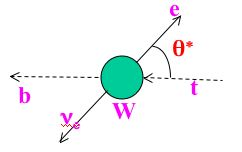
\includegraphics[width = 0.4 \textwidth]{Chapters/Chapter1_SM/Figures/image_cos_theta_cartoon.jpg}
 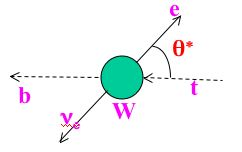
\includegraphics[width = 0.4 \textwidth]{Chapters/Chapter1_SM/Figures/CosThetaImage.png}
 \caption{\textit{Will need to find a beter image otherwise this doesn't make sense to show ...}}
\end{figure}


